% GENERATED by tools/make_figures.py — do not edit.
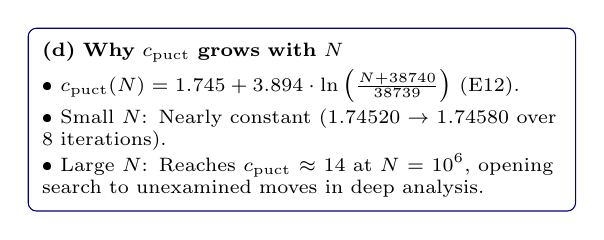
\begin{tikzpicture}
  \node[draw=NavyBlue, fill=white, rounded corners=3pt, inner sep=5pt, text width=66mm, font=\scriptsize, align=left] (box) {
    \textbf{(d) Why $c_{\mathrm{puct}}$ grows with $N$}\\[0.6ex]
    • $c_{\mathrm{puct}}(N) = 1.745 + 3.894\cdot \ln\left(\frac{N+38740}{38739}\right)$ (E12).\\[0.4ex]
    • Small $N$: Nearly constant ($1.74520 \to 1.74580$ over 8 iterations).\\[0.4ex]
    • Large $N$: Reaches $c_{\mathrm{puct}} \approx 14$ at $N=10^6$, opening search to unexamined moves in deep analysis.
  };
\end{tikzpicture}
